% This is "sig-alternate.tex" V2.1 April 2013
% This file should be compiled with V2.5 of "sig-alternate.cls" May 2012
%
% This example file demonstrates the use of the 'sig-alternate.cls'
% V2.5 LaTeX2e document class file. It is for those submitting
% articles to ACM Conference Proceedings WHO DO NOT WISH TO
% STRICTLY ADHERE TO THE SIGS (PUBS-BOARD-ENDORSED) STYLE.
% The 'sig-alternate.cls' file will produce a similar-looking,
% albeit, 'tighter' paper resulting in, invariably, fewer pages.
%
% ----------------------------------------------------------------------------------------------------------------
% This .tex file (and associated .cls V2.5) produces:
%       1) The Permission Statement
%       2) The Conference (location) Info information
%       3) The Copyright Line with ACM data
%       4) NO page numbers
%
% as against the acm_proc_article-sp.cls file which
% DOES NOT produce 1) thru' 3) above.
%
% Using 'sig-alternate.cls' you have control, however, from within
% the source .tex file, over both the CopyrightYear
% (defaulted to 200X) and the ACM Copyright Data
% (defaulted to X-XXXXX-XX-X/XX/XX).
% e.g.
% \CopyrightYear{2007} will cause 2007 to appear in the copyright line.
% \crdata{0-12345-67-8/90/12} will cause 0-12345-67-8/90/12 to appear in the copyright line.
%
% ---------------------------------------------------------------------------------------------------------------
% This .tex source is an example which *does* use
% the .bib file (from which the .bbl file % is produced).
% REMEMBER HOWEVER: After having produced the .bbl file,
% and prior to final submission, you *NEED* to 'insert'
% your .bbl file into your source .tex file so as to provide
% ONE 'self-contained' source file.
%
% ================= IF YOU HAVE QUESTIONS =======================
% Questions regarding the SIGS styles, SIGS policies and
% procedures, Conferences etc. should be sent to
% Adrienne Griscti (griscti@acm.org)
%
% Technical questions _only_ to
% Gerald Murray (murray@hq.acm.org)
% ===============================================================
%
% For tracking purposes - this is V2.0 - May 2012

\documentclass{sig-alternate-05-2015}


\begin{document}

% Copyright
%\setcopyright{acmcopyright}
%\setcopyright{acmlicensed}
%\setcopyright{rightsretained}
%\setcopyright{usgov}
%\setcopyright{usgovmixed}
%\setcopyright{cagov}
%\setcopyright{cagovmixed}


% DOI
\doi{DOI}

% ISBN
\isbn{ISBN}

%Conference
\conferenceinfo{SEMANTICS '17}{September 16--19, 2017, Amsterdam, The Netherlands}

\acmPrice{\$0.00}

%
% --- Author Metadata here ---
\conferenceinfo{SEMANTICS}{'2017 Amsterdam, The Netherlands}
%\CopyrightYear{2007} % Allows default copyright year (20XX) to be over-ridden - IF NEED BE.
%\crdata{0-12345-67-8/90/01}  % Allows default copyright data (0-89791-88-6/97/05) to be over-ridden - IF NEED BE.
% --- End of Author Metadata ---

\title{Towards IoT platforms' integration: Semantic Translations between {\ttlit W3C SSN} and {\ttlit ETSI SAREF}}

%
% You need the command \numberofauthors to handle the 'placement
% and alignment' of the authors beneath the title.
%
% For aesthetic reasons, we recommend 'three authors at a time'
% i.e. three 'name/affiliation blocks' be placed beneath the title.
%
% NOTE: You are NOT restricted in how many 'rows' of
% "name/affiliations" may appear. We just ask that you restrict
% the number of 'columns' to three.
%
% Because of the available 'opening page real-estate'
% we ask you to refrain from putting more than six authors
% (two rows with three columns) beneath the article title.
% More than six makes the first-page appear very cluttered indeed.
%
% Use the \alignauthor commands to handle the names
% and affiliations for an 'aesthetic maximum' of six authors.
% Add names, affiliations, addresses for
% the seventh etc. author(s) as the argument for the
% \additionalauthors command.
% These 'additional authors' will be output/set for you
% without further effort on your part as the last section in
% the body of your article BEFORE References or any Appendices.

\numberofauthors{9} %  in this sample file, there are a *total*
% of EIGHT authors. SIX appear on the 'first-page' (for formatting
% reasons) and the remaining two appear in the \additionalauthors section.
%
\author{
% You can go ahead and credit any number of authors here,
% e.g. one 'row of three' or two rows (consisting of one row of three
% and a second row of one, two or three).
%
% The command \alignauthor (no curly braces needed) should
% precede each author name, affiliation/snail-mail address and
% e-mail address. Additionally, tag each line of
% affiliation/address with \affaddr, and tag the
% e-mail address with \email.
%
% 1st. author
\alignauthor
João Moreira\\
       \affaddr{University of Twente}\\
       \affaddr{Enschede, The Netherlands}\\
       \email{j.luizrebelomoreira@utwente.nl}
% 2nd. author
\alignauthor
Laura Danielle\\
       \affaddr{TNO}\\
       \affaddr{The Haugue, The Netherlands}\\
       \email{webmaster@marysville-ohio.com}
% 3rd. author
\alignauthor 
Luis Ferreira Pires\\
       \affaddr{University of Twente}\\
       \affaddr{Enschede, The Netherlands}\\
       \email{larst@affiliation.org}
\and  % use '\and' if you need 'another row' of author names
% 4th. author
\alignauthor 
Marten van Sinderen\\
       \affaddr{University of Twente}\\
       \affaddr{Enschede, The Netherlands}\\
       \email{lleipuner@researchlabs.org}
% 5th. author
\alignauthor 
Katarzyna Wasielewska\\
       \affaddr{Systems Research Institute, Polish Academy of Sciences}\\
       \affaddr{Warsaw, Poland}\\
       \email{katarzyna.wasielewsk@ibspan.waw.pl}
% 6th. author
\alignauthor 
Pawel Szmeja\\
       \affaddr{Systems Research Institute, Polish Academy of Sciences}\\
       \affaddr{Warsaw, Poland}\\
       \email{fogartys@amesres.org}
\and  % use '\and' if you need 'another row' of author names
% 7th. author
\alignauthor 
Wieslaw Pawlowski\\
       \affaddr{Systems Research Institute, Polish Academy of Sciences}\\
       \affaddr{Warsaw, Poland}\\
       \email{lleipuner@researchlabs.org}
% 8th. author
\alignauthor 
Maria Ganzha\\
       \affaddr{Systems Research Institute, Polish Academy of Sciences}\\
       \affaddr{Warsaw, Poland}\\
       \email{fogartys@amesres.org}
% 9th. author
\alignauthor 
Marcin Paprzycki\\
       \affaddr{Systems Research Institute, Polish Academy of Sciences}\\
       \affaddr{Warsaw, Poland}\\
       \email{fogartys@amesres.org}
}
% There's nothing stopping you putting the seventh, eighth, etc.
% author on the opening page (as the 'third row') but we ask,
% for aesthetic reasons that you place these 'additional authors'
% in the \additional authors block, viz.
%\additionalauthors{Additional authors: John Smith (The Th{\o}rv{\"a}ld Group,
%email: {\texttt{jsmith@affiliation.org}}) and Julius P.~Kumquat
%(The Kumquat Consortium, email: {\texttt{jpkumquat@consortium.net}}).}
%\date{30 July 1999}
% Just remember to make sure that the TOTAL number of authors
% is the number that will appear on the first page PLUS the
% number that will appear in the \additionalauthors section.

\maketitle
\begin{abstract}
Several IoT ontologies were developed to promote semantic interoperability of IoT solutions. The most notable ontology, the W3C Semantic Sensor Network (SSN), is considered an ontological foundation for diverse IoT initiatives, as OpenIoT. With characteristics similar to SSN, the ETSI Smart Appliances REFerence (SAREF) ontology emphasizes the needs of smart home solutions. Some IoT solutions rely on platform-specific ontologies and their integration requires mechanisms to align these ontologies. In this paper we describe the initial steps towards an alignment between SSN and SAREF, proposing an initial specification of the translation mappings among the main elements of the ontologies, i.e. classes, object properties and data properties. The alignment will be used in a semantic translation process leveraging the INTER-IoT project. An initial evaluation of the translation demonstrates how a wind sensor (Vaisala WM30), an example provided by the W3C, is translated from SSN to SAREF.
\end{abstract}


%
% The code below should be generated by the tool at
% http://dl.acm.org/ccs.cfm
% Please copy and paste the code instead of the example below. 
%
\begin{CCSXML}
<ccs2012>
<concept>
<concept_id>10002951.10003260.10003309.10003315</concept_id>
<concept_desc>Information systems~Semantic web description languages</concept_desc>
<concept_significance>500</concept_significance>
</concept>
</ccs2012>
\end{CCSXML}

\ccsdesc[500]{Information systems~Semantic web description languages}


%
% End generated code
%

%
%  Use this command to print the description
%
\printccsdesc

% We no longer use \terms command
%\terms{Theory}

\keywords{Semantic interoperability, internet-of-things, ontology alignment, SAREF, W3C SSN}

\section{Introduction}
- Problem context, Goal/Requirement:\\
- Proposal:\\
- Validation:\\ 
- Paper structure:\\ 
Over the last years a number of IoT ontologies were proposed to achieve semantic interoperability of sensors in integrated IoT solutions. In this context, the W3C Semantic Sensor Network (SSN) is considered an ontological basis for the IoT, covering any application of sensors, being used as foundation by several initiatives (e.g. OpenIoT). Recently, the ETSI Smart Appliances REFerence (SAREF) ontology was developed, targeting smart home solutions. It is based on several “assets”, i.e. syntactic standards, proprietary data models and other ontologies, as W3C SSN. To enable integration among two IoT platforms, where one platform relies on SSN and the other relies on SAREF, an ontology alignment mechanism between SSN and SAREF is required. In this paper we describe the initial steps towards bi-directional semantic translation rules between SSN and SAREF. The approach makes use of ontology engineering to specify these translations. This specification will be further configured and deployed in the Inter Platform Semantic Mediator (IPSM) of the INTER-IoT project. These initial steps include the bi-directional mappings among the main elements of the ontologies, i.e. classes, object properties and data properties. An initial evaluation of the translation is presented, demonstrating how the wind sensor WM30, an example provided by the W3C, is translated from SSN to SAREF.

\section{BACKGROUND}

\subsection{INTER-IoT semantic mediator}
The H2020 project Interoperability of Heterogeneous IoT Platforms (INTER-IoT) [1, 2] is currently developing the  Inter-Platform Semantic Mediator (IPSM) tool. The following tasks are executed as part of the IPSM design and implementationto:  (2) develop a central modular ontology, consisting of a core IoT ontology and domain specific modules, (3) preparealignments between ontologies of communicating artefacts and the central ontology,  (4) use the alignments for translations, and (5) establish a multi-channel (1-1, 1-many, many-1) communication architecture that will facilitate translations in all needed contexts. While complete ontologies are used to “build semantic understanding”, only conversation-specific alignments are stored and used for actual translations. Figure X illustrates IPSM architecture. Ontology alignments and translation channels can be managed and ontology reconciliation  through the REST Manager.

IPSM core: Channel Manager, Semantic Translation Channels, Alignment Applicators \\
IPSM alignments repository: I/O Alignments, Converters \\
IPSM communication infrastructure: Communication channels, Semantic Annotators \\

INTER-IoT.D4.1[Figure 107: Functional Components of the INTER-IoT RA with the components of the Data and Semantics interoperability layer of the INTER-LAYER\\

\begin{figure}
\centering
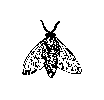
\includegraphics[height=1in, width=1in]{fly}
\caption{Inter-Platform Semantic Mediator}
\end{figure}

Ontology alignment – semantic translations [3]

Semantic translation supported by IPSM uses ontology alignments that are specified in a dedicated format….. 


\subsection{W3C Semantic Sensor Network}
The SSN ontology is an ontology developed by W3C and the last version was published in 2011 in the official URL (https://www.w3.org/2005/Incubator/ssn/ssnx/ssn). It provides a framework to describe sensors, devices, observations and related concepts, enabling reasoning either about individual sensors as well as about the connection of a set of sensors. 

A ‘sensing device’ is a sensor that reports measurements and observations of real world phenomena. A sensor is different in nature from other types of devices, e.g. actuators, because of its event-based behavior, which requires temporal relationships. SSN enables reasoning about the measurements that can ease the development of advanced applications, for example by reasoning about sensor measurements, considering constraints as power restriction and limited memory. 

The SSN ontology is composed of modules and is grounded in the foundational ontology DOLCE Ultra-Light (DUL). The modules we are covering in this paper are the following:
DUL module: represents the foundational categorization of Designed Artifact, Method, Physical Object, Quality, Region and Situation.  

Skeleton module: represents the most basic concepts regarding sensors, as abstractions of real world phenomena that describe input and output of sensing, properties, observations and features of interest.

System module: represents the system concept as a Physical Object (DUL) composed by other systems (hasSubSystem), which has deployment(s) (hasDeployment), normal operating environment(s) (hasOperatingRange), survival range(s) (hasSurvivalRange) and location(s) relative to other entities (onPlatform).

Process module: Input, Output, Process, hasInput, hasOutput, isProducedBy

Measuring module: SensingDevice, SensorDataSheet, observes

Measuring Capability module: Accuracy, DetectionLimit, Drift, Frequency, Latency, MeasurementCapability, MeasurementProperty, MeasurementRange, Precision, Resolution, ResponseTime, Selectivity, Sensitivity	hasMeasurementCapability, hasMeasurementProperty

Observation module: represents a situation with a discrete time instant or a period assigned to a phenomenon, involving the application of a specified procedure, e.g. a process chain. The result of an observation is an estimate of the value of a property of some feature, allowing observation data using different procedures to be combined unambiguously. 

Device module: device

The W3C SSN Incubator Group created an example of the use of SSN by describing the Vaisala WM30 wind sensor (https://www.w3.org/2005/Incubator/ssn/ssnx/meteo/WM30.html). It describes the measurement capabilities, power supply and operating and survival properties based on the technical specification about the measurement of wind direction and speed. This example was initially reported in [4], which gives a precise description of the WM30 sensor. However, the axioms representing its main definitions and restrictions are different, following the changes in the TBox of SSN over the past years. Bellow we update these main definitions:
\\




\subsection{ETSI Smart Appliances REFerence}
The SAREF ontology [5] is a reference model that facilitates the matching of existing assets, e.g. standards, ontologies, data models and protocols, in the smart appliances domain. 

The SAREF ontology provides building blocks that enables reutilization of different parts of the ontology according to specific requirements. One of these assets is SSN, which inspired the creation of the main elements of SAREF: Device, Sensor, Unit of Measure and Time/Duration. 

A device (e.g. a switch) represents tangible objects designed to accomplish one or more functions in diverse types of locations (e.g. households, buildings). The SAREF ontology offers a lists of basic functions that can be combined towards more complex functions in a single device. For example, a switch offers an actuating function of type “switching on/off”. 

Each function has some associated commands, which can also be picked up as building blocks from a list. For example, the “switching on/off” is associated with the commands “switch on”, “switch off” and “toggle”. Depending on the function(s) it accomplishes, a device can be found in some corresponding states that are also listed as building blocks. 

A Device offers a Service, which  is a representation of a Function to a network that makes the function discoverable, registerable and remotely controllable by other devices in the network. A Service can represent one or more functions. A Service is offered by a device that wants (a certain set of) its function(s) to be discoverable, registerable, remotely controllable by other devices in the network. A Service must specify the device that is offering the service, the function(s) to be represented, and the (input and output) parameters necessary to operate the service. 

A Device in the SAREF ontology is also characterized by an (Energy/Power) Profile that can be used to optimize the energy efficiency in a home or office that are part of a building.


\section{METHODOLOGY}
The development of the bi-directional semantic translations follows a common software engineering approach, considering a specification and an implementation phase during design time. 

Specification: 

Implementation: configuration within IPSM.

This approach enables to (re)use the specification for different strategies of ontology alignments’ implementation, e.g. matching, mapping, and merging. In this paper we present part of the specification, referring to the unidirectional semantic translation from SSN to SAREF.

As first evaluation of this specification, we simulate an unidirectional semantic translation from WM30 ontology, represented as an extension of SSN, to an ontology represented as SAREF. In general, the result from the translations must represent the WM30 wind sensor with SAREF, keeping similar semantics of the original. 

Therefore, the goal of this evaluation is to check the semantic similarity between the original and the final ontologies. Here we used an approach based on competency questions to measure this similarity. A list of competency questions is presented and each question is responded by querying the elements (classes, properties and instances) of both ontologies. The responses are compared to verify whether the semantics is maintained after executing the translation. Intentionally, the competency questions were conceived according to the expressiveness of the SSN WM30 ontology, targeting its main elements, as the different measurement capabilities illustrated in the technical specifications (Figure X).

\begin{figure}
\centering
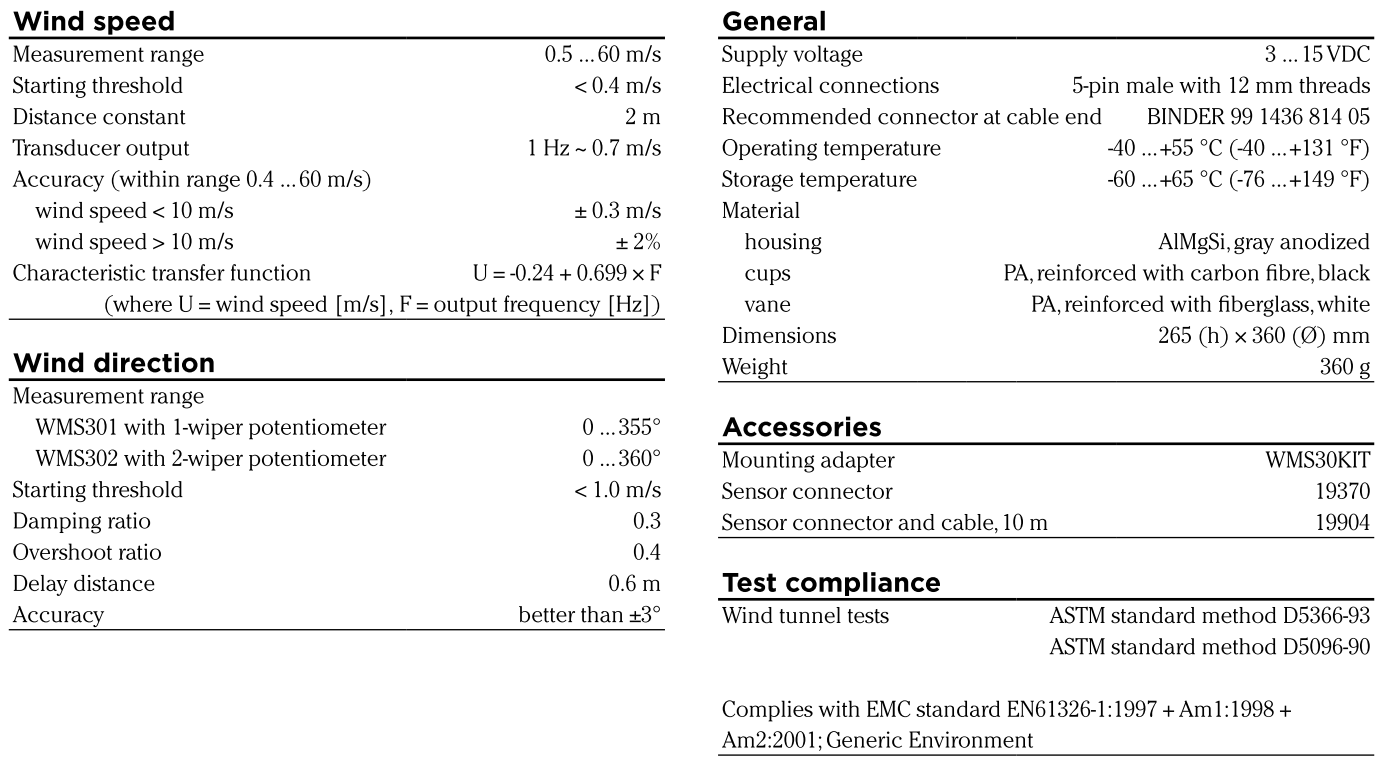
\includegraphics[height=1in, width=1in]{WM30specifications}
\caption{Inter-Platform Semantic Mediator}
\end{figure}

Competency questions: 
\\CQ01. What are the main characteristics of the Vaisala WM30 sensor? 
\\CQ02. What is the composition of this sensor, i.e. what other devices are part of WM30?
\\CQ03. What measurement properties this sensor provides?
\\CQ04. What are the accuracy, delay distance, starting threshold and damping ratio of WMS30 wind direction sensors? \\CQ05. What measurement range constraints differentiate these types of wind direction sensors?
\\CQ06. What are the distance constant, starting threshold and transducer output of wind speed sensors? 
\\CQ07. What are the ranges of accuracy and condition ranges  constraints differentiate these types of wind speed sensors?
\\CQ08. What is the characteristic transfer function of WM30?



\section{SEMANTIC TRANSLATIONS}

\subsection{Mappings}
Mappings between SSN and SAREF were specified through an ontological analysis of their TBox, i.e. concepts and roles definitions (predicates) with logical operations. A study was made on how SSN and SAREF describe the characteristics of sensors and their measurements. 

The mappings follow a logic sequence according to the main elements and similar structures of SSN and SAREF. Here we detail only the mappings from SSN to SAREF because of space limitation – the other direction, from SAREF to SSN, will be reported in the future. For each mapping a code snippet is presented, as a pseudo-code, to illustrate the creation of the ontology based on SAREF.

While the main element in SSN is the Sensing Device, which is a subclass of Device and Sensor, in SAREF the main element is Device. 

M01: The characteristics of ssn:SensingDevice, inherited from ssn:Sensor and ssn:System, is mapped to saref:Sensor, which inherits saref:Device properties, including the relationship with the saref:SensingFunction (saref:hasFunction). The code snippet below illustrates this mapping.   

<CS01>Code snippet 01

Figure X illustrates the elements involved in this mapping. Notice that, indirectly, this mapping also transforms from ssn:Sensor to saref:Sensor.

\begin{figure}
\centering
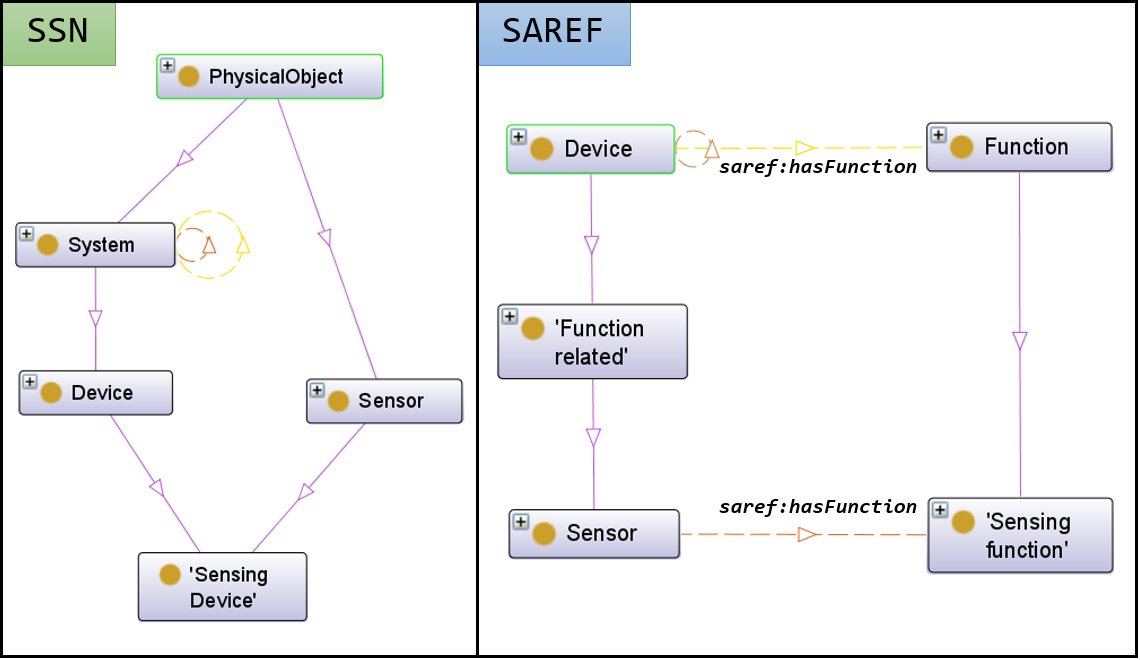
\includegraphics[height=1in, width=1in]{SSN_SAREF_SensingDevice_Device}
\caption{Inter-Platform Semantic Mediator}
\end{figure}


M02: Once executing M01, the next step is to check the composition relationship of a device, i.e. the components that are part of a device, which are characterized by both SSN and SAREF. In SSN, the object property ssn:hasSubSystem relating two ssn:System represents this relationship. In SAREF, the object property saref:consistsOf plays this role, relating two saref:Device in a similar way, both illustrated in Figure X as a self-relationship. 

Therefore, when ssn:hasSubSystem is used between the ssn\_sensingDevice (from M01) and a ssn:System, which must be a ssn:Device or a ssn:SensingDevice, then it is mapped to saref:consistsOf object property of the saref\_sensor (from M01). If the device component is a ssn:SensingDevice, then a recursive algorithm is used by applying M01 to it. If the device component is a ssn:Device, then it is created a saref:Device. The code snippet below illustrates this mapping.

<CS02>Code snippet 02

M03: ssn:observes  saref:measuresProperty
Ssn:Property  saref:Property

M04: ssn:MeasurementCapability
saref:UnitOfMeasure + saref:Property

M05: ssn:Sensing (ssn:Process)
saref:SensingFunction

\subsection{Evaluation}
The translation output, i.e. the WM30 ontology according to SAREF, in OWL, is available in (github link). For each question, at first we answer based on the original (SSN) and, then, we answer the same question for the final (SAREF). Second, we compare whether the semantics of the response is similar to each other, ranking this similarity with four possible values: (1) cannot answer; (2) semantics is lost, representing an important gap; (3) semantics is lost, but covers the main elements; (4) semantics is totally maintained. At last, the ranks are summed and the overall maintained semantics is calculated.

To respond each question it was used an ontology editor (Protegé and TopBraid Composer Free) to navigate and/or query (SPARQL) over the ontology. 

Responding the competency questions:
CQ01. In the original ontology (SSN), the main characteristics of the Vaisala WM30 sensor can be extracted by starting the navigation in the WM30:Vaisala\_WM30 element, which is a ssn:SensingDevice, inheriting the properties from ssn:Device and ssn:Sensor. Besides, the rdfs:comment with a general description of this wind sensor, it represents that the sensor is composed by two sensors (WM30:WM30\_WindDirection and WM30:WM30\_WindSpeed), one for wind direction and another for wind speed (both ssn:Sensor). Moreover, WM30 can observe (measure) the types (properties) WM30:WindDirection and WM30:WindSpeed (both ssn:Property). Figure X illustrates these properties.

\begin{figure}
\centering
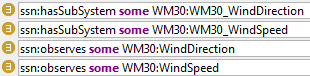
\includegraphics[height=1in, width=1in]{SSN_SystemProperties}
\caption{Inter-Platform Semantic Mediator}
\end{figure}

In the generated ontology (SAREF), according to M01, WM30:Vaisala\_WM30 element is created as a saref:Sensor. A saref:SensingFunction (subclass or instance?) is created and the WM30:Vaisala\_WM30 element linked to it. 

Some issues were detected in this example:
\\First, saref:Sensor provides subclasses that are types of sensors, as saref:SmokeSensor and saref:TemperatureSensor, which have the properties of saref:hasFunction and saref:measuresProperty, linking the type of the sensor with functions it has and the type of property it measures, in these cases saref:Smoke and saref:Temperature, respectively. The correct implementation for the wind sensor would create the subclass saref:WindSensor, with function sensing and measuring the properties of wind direction and wind speed. 

Mappings M01 supported the creation of these elements.

CQ02.

CQ03.

CQ04.

CQ05.

CQ06.

CQ07. 

\subsection{Discussion}
SSN: why ssn:Sensor is not a ssn:System? At first, the dc:source property of ssn:Sensor states that: “allows sensors, methods, instruments, systems, algorithms and process chains as the process used of an observation (…) they are all grouped under the term sensor”. Second, by having ssn:Sensor as sub class of ssn:System, it inherits the composition relationship (ssn:hasSubSystem) and, thus, can represent a set of sensors.  

The problem when transforming WM30:WM30\_WindDirection as ssn:Sensor 

\section{CONCLUSIONS}

%ACKNOWLEDGMENTS are optional
\section{Acknowledgments}
This section is optional.

%
% The following two commands are all you need in the
% initial runs of your .tex file to
% produce the bibliography for the citations in your paper.
\bibliographystyle{abbrv}
\bibliography{sigproc}  % sigproc.bib is the name of the Bibliography in this case
% You must have a proper ".bib" file
%  and remember to run:
% latex bibtex latex latex
% to resolve all references
%
% ACM needs 'a single self-contained file'!
%
%APPENDICES are optional
%\balancecolumns




\end{document}
